\documentclass[9pt,a4paper]{extarticle}
\usepackage{elr-style}
\usepackage{graphicx}
\usepackage{booktabs}
\usepackage{array}
\usepackage{tabularx}
\usepackage{multicol}
\usepackage{amsmath}
\usepackage{float}
\usetikzlibrary{positioning,arrows.meta,fit}
\newcolumntype{L}{>{\raggedright\arraybackslash}X}

%% Figures live in figures/ next to this file (make_figures.py rebuilds the
%% plots and the enclosure render from the repository's data and STL files).
%% Flat uploads (e.g. Overleaf) also work.
\graphicspath{{figures/}{./}}

%% Values still to be filled in before submission print in red.
\newcommand{\tbd}[1]{{\color{red}\bfseries #1}}

%% Two-column body under the ELR header. Floats do not work inside multicols,
%% so figures and tables are placed in the flow with \captionof.
\usepackage{caption}
\newenvironment{colfig}
  {\par\vspace{0.5em}\noindent\begin{minipage}[t]{\linewidth}\centering}
  {\end{minipage}\par\vspace{0.5em}}

\setlength{\columnsep}{6mm}
\setlength{\multicolsep}{0pt}

%% =====================================================================
%% FINAL SHORT PAPER -- 3 pages of body; references and appendix after.
%% Compile with LuaLaTeX (twice, for the references); XeLaTeX works on Overleaf
%% but not on a Mac TeX Live without TeX Gyre Heros installed as a system font.
%% =====================================================================

\ELRArticleTitle{Prostart: Democratizing Sprint Training with a Low-Cost Reaction-Time and Photo-Finish System for Track \& Field}
\ELRAuthor{Arianna Bartocci, Duarte Chambel, Lorenzo Galli, Loke Enlund Östangård, Ninad Purekar}
\ELRAffiliation{KTH Royal Institute of Technology}
\ELREmail{Technology and Health Project Course - HT26}

\ELRAbstract{%
\fontsize{9}{11}\selectfont
Sprint races are decided by milliseconds, yet the systems that time reaction and finish are costly \cite{vsath} and stay with federations and large clubs, while everyone else times by hand.
We present Prostart: a start unit that mounts onto a standard starting block, and a phone app that turns a smartphone into a photo finish.
The unit, an ESP32-C3 with a BMI270 accelerometer sampled at 804~Hz on a custom PCB in a 3D-printed box, gives the start commands, finds the push-off with a threshold-independent two-stage onset picker, and sends the ``go'' instant over Bluetooth Low Energy (BLE) to the phone, which times the chest crossing the line with an on-device pose model, a synchronized clock and sub-frame interpolation. Against 240~fps video with an LED marking ``go'', reaction times agreed within about 8~ms, the uncertainty of the video reference itself; finish times agreed with a 60~fps reference within 10~ms, a third of our one-frame target (33~ms at 30~fps), whereas hand timing read about 0.24~s fast.
}

\ELRSeries{ELR}
\ELRPages{1}{1}

\begin{document}
\ELRMakeTitle

\begin{multicols}{2}
\raggedcolumns
\setstretch{1.02}
\titleformat{\section}{\sffamily\fontsize{12}{14}\selectfont\bfseries\color{ELRBlue}}{\ELRAccentText{\thesection}}{0.6em}{}
\titlespacing*{\section}{0pt}{0.8em}{0.3em}

%% =====================================================================
\section{Introduction}
%% =====================================================================

In competitive sprinting, athletes train for years to gain a few hundredths of a second: Noah Lyles won the Paris 2024 Olympic 100~m final by five thousandths \cite{olymp}. Reaction times differ by several hundredths between elite sprinters \cite{lipps}, so part of the winning margin is decided before the athlete has even moved. Reaction time runs from the starting signal to the first force on the block; under 0.100~s is a false start, a limit based on the minimum auditory reaction time \cite{pain}, and the fastest valid Olympic reactions lie just above it \cite{lipps,brosnan}. The systems that measure it are installed at certified meets \cite{lynx}, and even a single-block training version lists at about US\$1{,}600 \cite{vsath}. Coaches therefore time by hand, which reads about 0.24~s faster than electronic timing \cite{mann}: an error larger than the gains an athlete trains for.

Photocells start when the torso breaks a beam, so their times exclude the reaction \cite{haugen}. FinishLynx ReacTime measures reaction to 1/1000~s from a sensor on every block \cite{lynx}; its patent detects the onset when acceleration crosses a threshold \cite{lynxpatent}, which by construction reports it late. Omega samples the force on the footrest at 4~kHz and pairs it with a finish camera of up to 40{,}000 images per second \cite{omega}, and earlier student work used load cells, robust in 18 of 20 starts but without a timing-accuracy characterization \cite{heim}. All of these are either costly or built into the block, leaving a gap for a low-cost, portable system with a documented error budget.

This paper contributes (i)~a start unit on one microcontroller, from schematic to PCB to printed enclosure, whose onset picker is independent of its threshold; (ii)~a Flutter app that mirrors the start and turns the phone camera into a photo finish, synchronized to the unit over BLE; and (iii)~a validation of both against high-speed video, with every error term named. The unit started as a breadboard prototype (Appendix~\ref{app:hw}) and is now a complete system: the unit in its printed box and the app (Figure~\ref{fig:evolution}).

\begin{colfig}
  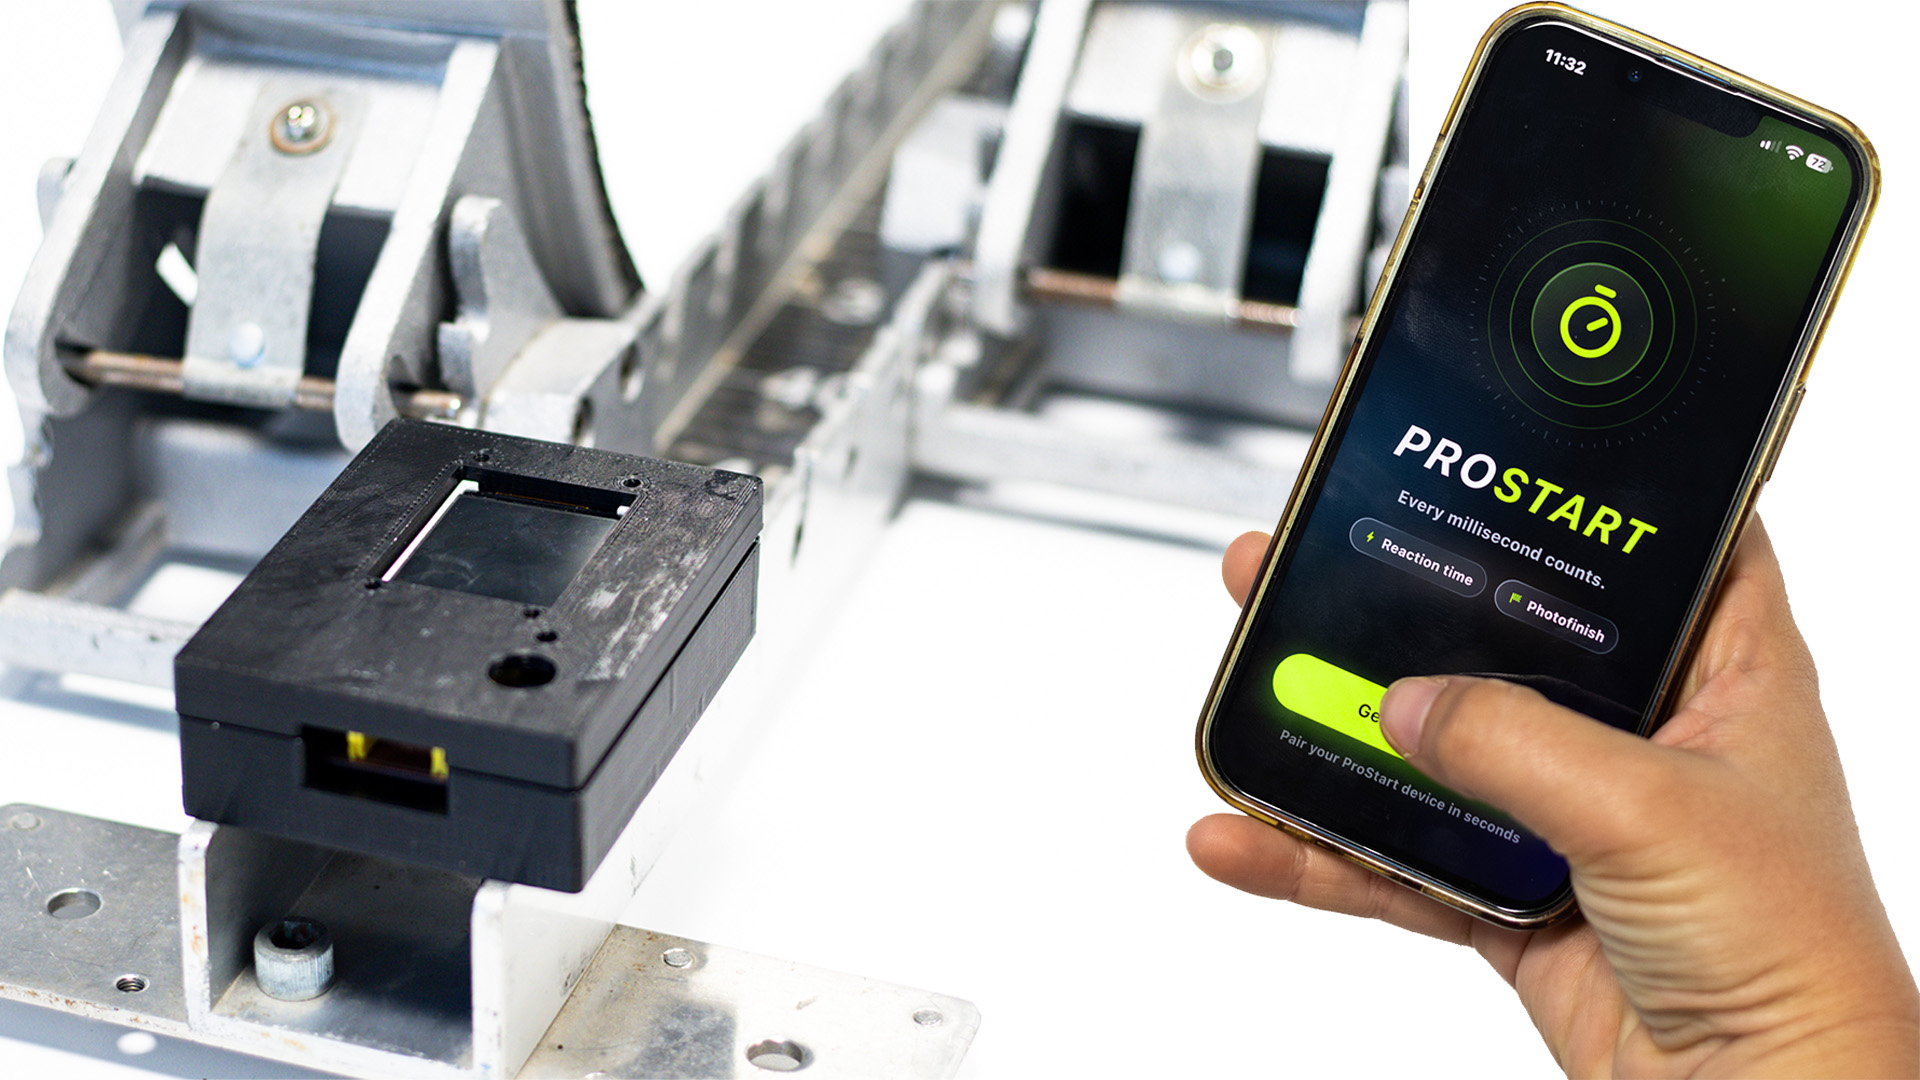
\includegraphics[width=\linewidth]{unit-app.jpg}\hfill
  \captionof{figure}{The complete system: the start unit in its printed box on the block (left) and the app (right).}
  \label{fig:evolution}
\end{colfig}

%% =====================================================================
\section{System design}
%% =====================================================================

\paragraph{Architecture.}
The system has two devices joined by one radio link (Figure~\ref{fig:arch}). The start unit sounds the commands, stamps them and the push-off on its own clock, and decides the verdict. The phone, standing at the finish, mirrors the start and times the finish. The microcontroller at the start reads the accelerometer and runs the radio. Each reading is timestamped in an interrupt and buffered in the sensor's FIFO, so Bluetooth traffic can delay it but never silently shift or lose a reading. A direct BLE link covers about 30~m, enough for start and acceleration work; for a full 100~m we plan a second ESP32-C3 at the finish, linked to the start unit over long-range ESP-NOW, which we field-tested beyond 100~m, and to the phone over BLE.

\begin{colfig}
\begin{tikzpicture}[font=\sffamily\scriptsize, node distance=3.2mm,
  blk/.style={draw=ELRBlue, fill=ELRBlueMist, rounded corners=1.5pt, align=center, inner sep=2.5pt, minimum height=5mm},
  grp/.style={draw=ELRGold, dashed, rounded corners=3pt, inner sep=3pt},
  arr/.style={-{Latex[length=1.6mm]}, draw=ELRDeepBlue, line width=0.5pt}]
  \node[blk] (imu) {BMI270\\804 Hz, $\pm$16 g};
  \node[blk, below=of imu] (mcu) {ESP32-C3\\ISR stamps 1 $\mu$s};
  \node[blk, below=of mcu, xshift=-5.5mm] (bz) {piezo\\4 kHz};
  \node[blk, below=of mcu, xshift=5.5mm] (ui) {TFT +\\button};
  \draw[arr] (imu) -- node[left, font=\sffamily\tiny]{FIFO} (mcu);
  \draw[arr] (mcu.south -| bz) -- (bz); \draw[arr,<->] (mcu.south -| ui) -- (ui);
  \node[grp, fit=(imu)(mcu)(bz)(ui), label={[text=ELRGold]above:start unit (on the block)}] (su) {};
  \node[blk, right=19mm of imu] (cam) {camera\\240 fps, 1/1000 s};
  \node[blk, below=of cam] (mp) {MediaPipe Pose\\chest front};
  \node[blk, below=of mp] (judge) {crossing, interp.\\$t_\mathrm{fin}-t_\mathrm{go}$};
  \draw[arr] (cam) -- (mp); \draw[arr] (mp) -- (judge);
  \node[grp, fit=(cam)(mp)(judge), label={[text=ELRGold]above:phone app (at the finish)}] (ph) {};
  \draw[arr] ([yshift=3mm]su.east) -- node[above, align=center]{events\\marks, set, go,\\result} ([yshift=3mm]ph.west);
  \draw[arr, <->] ([yshift=-5mm]su.east) -- node[below, align=center]{BLE ping/pong\\clock sync} ([yshift=-5mm]ph.west);
\end{tikzpicture}
\captionof{figure}{System overview. The start unit judges the start; the phone gets the ``go'' on its clock and times the finish.}
\label{fig:arch}
\end{colfig}

\paragraph{Hardware.}
A two-layer PCB (65.5$\times$34~mm, Appendix~\ref{app:hw}) carries an ESP32-C3 SuperMini, a BMI270 accelerometer breakout on I$^2$C at 400~kHz with its data-ready line on an interrupt pin, a 1.77'' display on SPI, a push button, and a 12 mm passive piezo. The unit runs from a USB power bank through the SuperMini's USB-C port. The enclosure, 75$\times$99.5$\times$25~mm, was designed around the board and printed in three parts (Figure~\ref{fig:boxmain}, left): a box with standoffs for the PCB, a lid with cutouts for the display and for the buzzer, and a button cap. Lastly a standard strap holds the box to the block's rail. Figure~\ref{fig:boxmain} (right) shows the assembled board mounted on the standoffs inside the printed box.

\begin{colfig}
  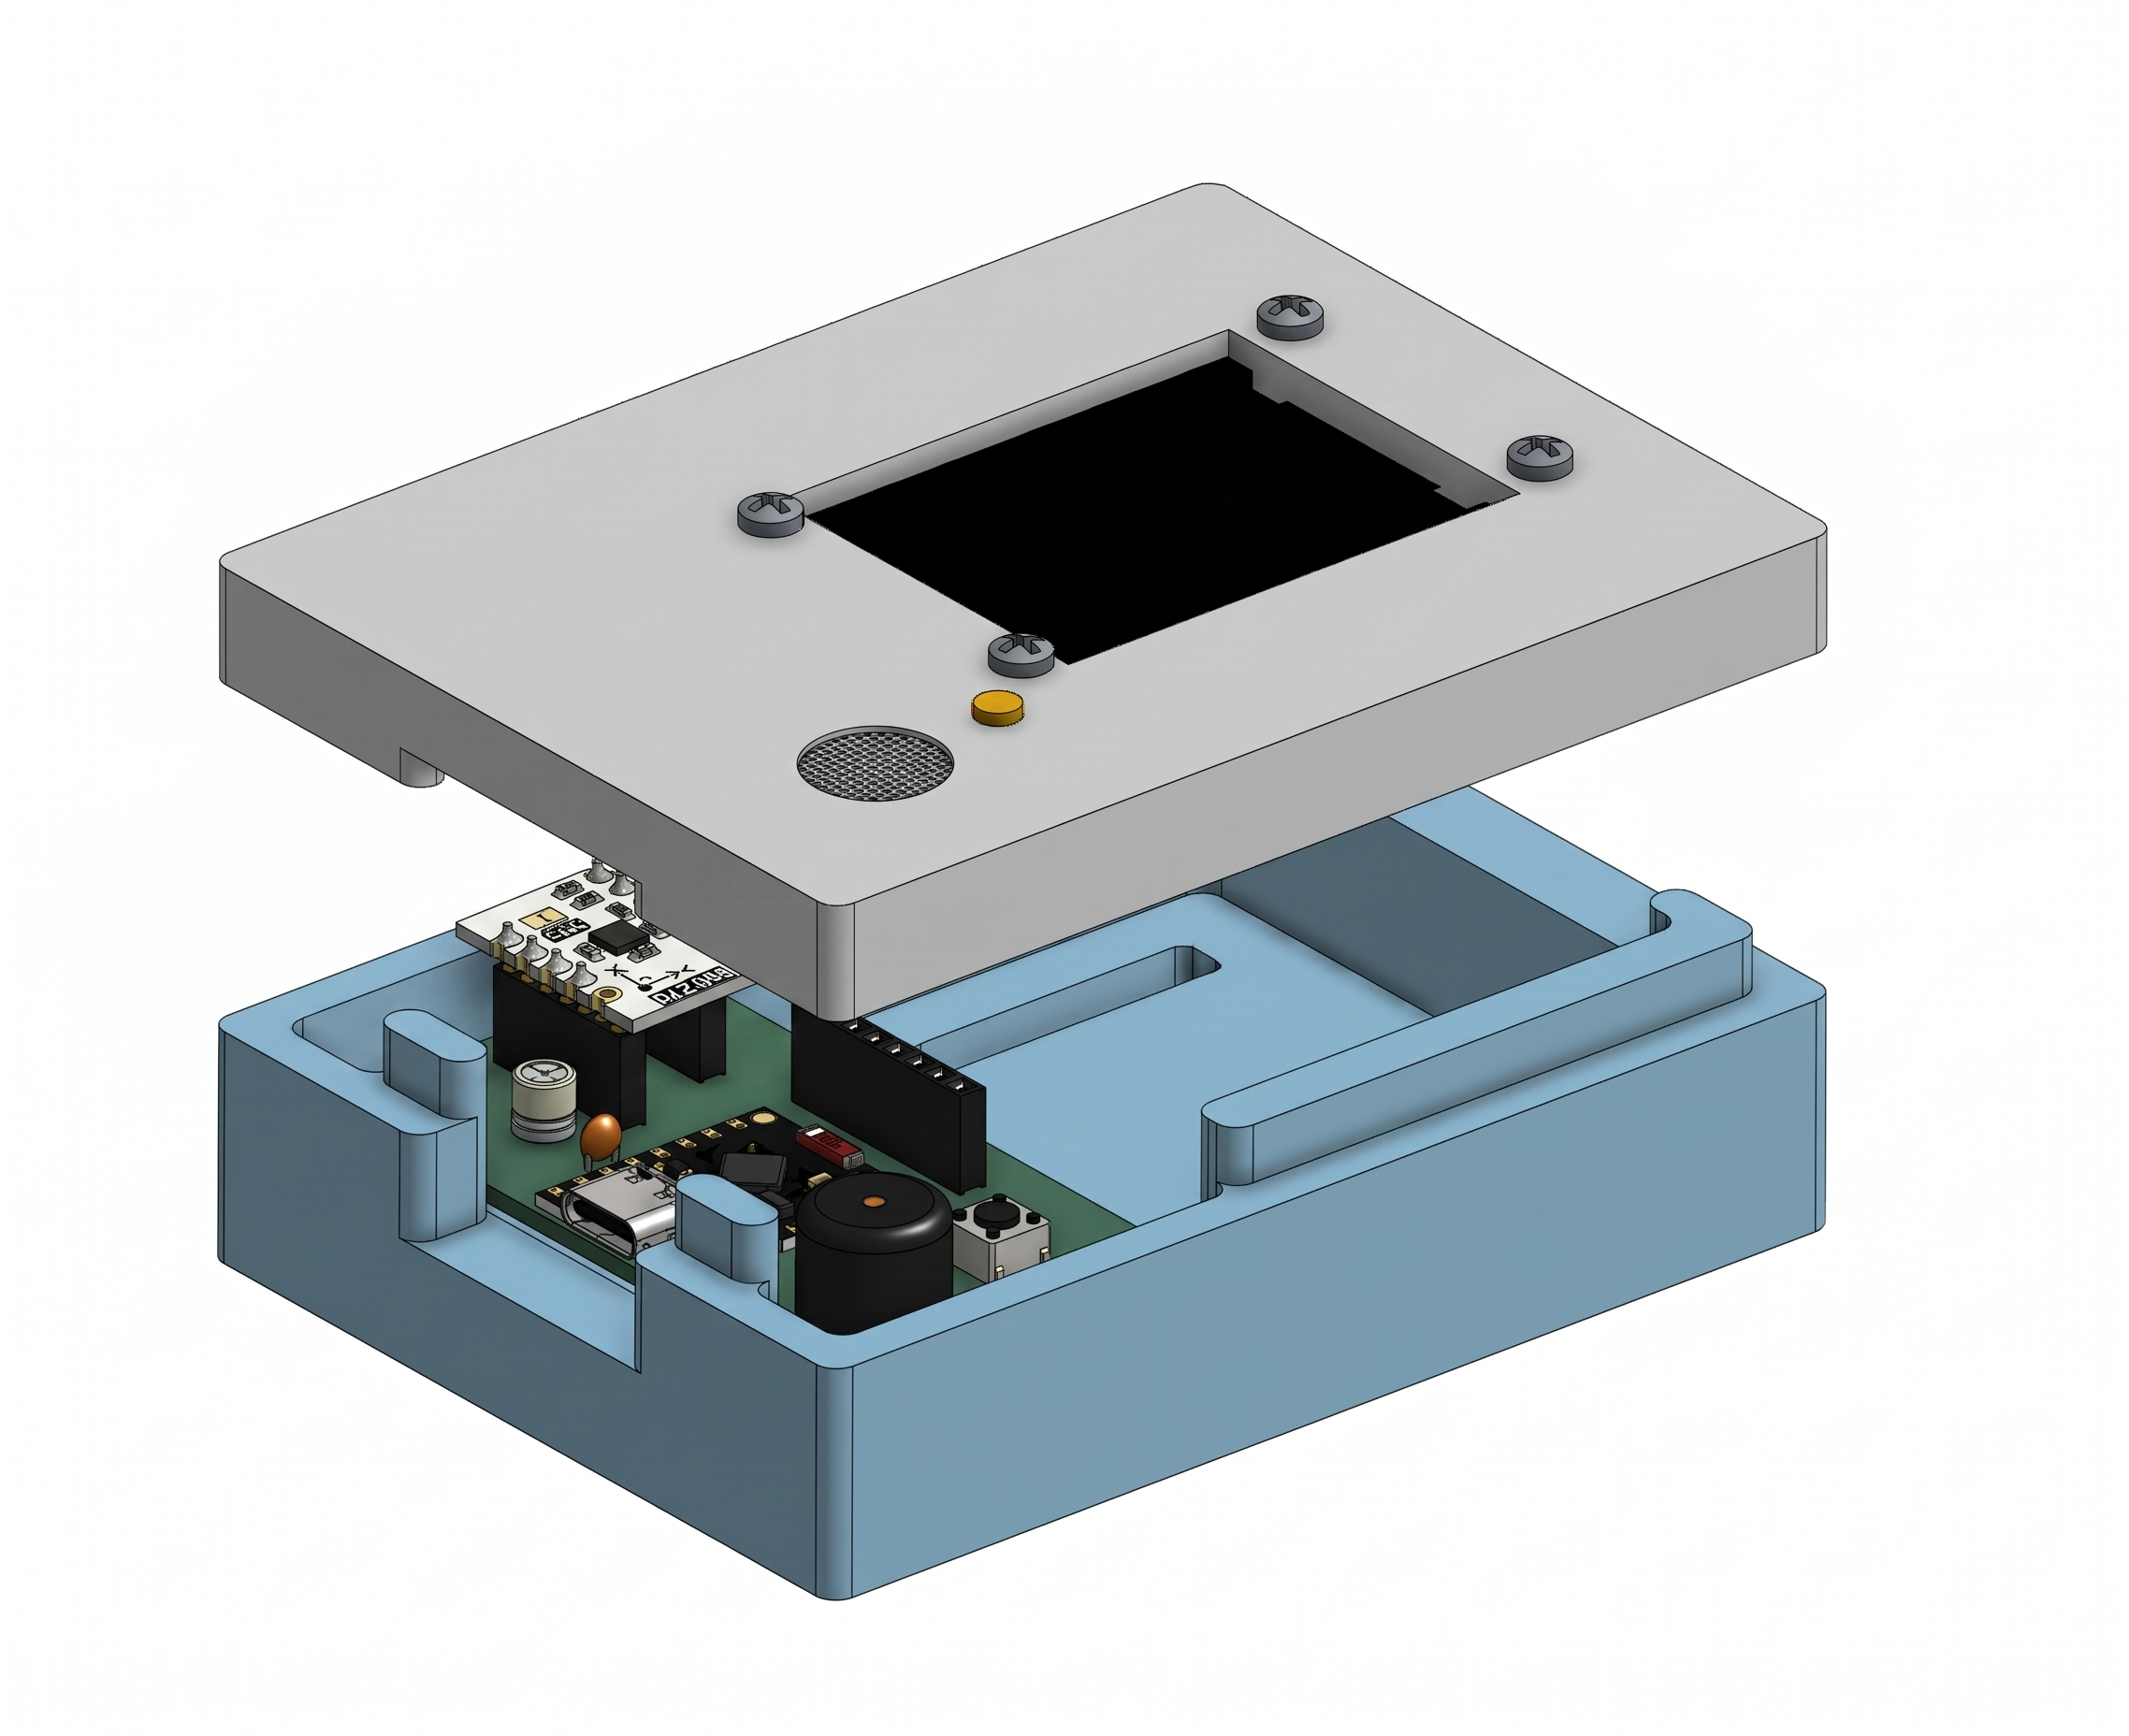
\includegraphics[width=0.49\linewidth]{figures/fig-box(2).jpeg}\hfill
  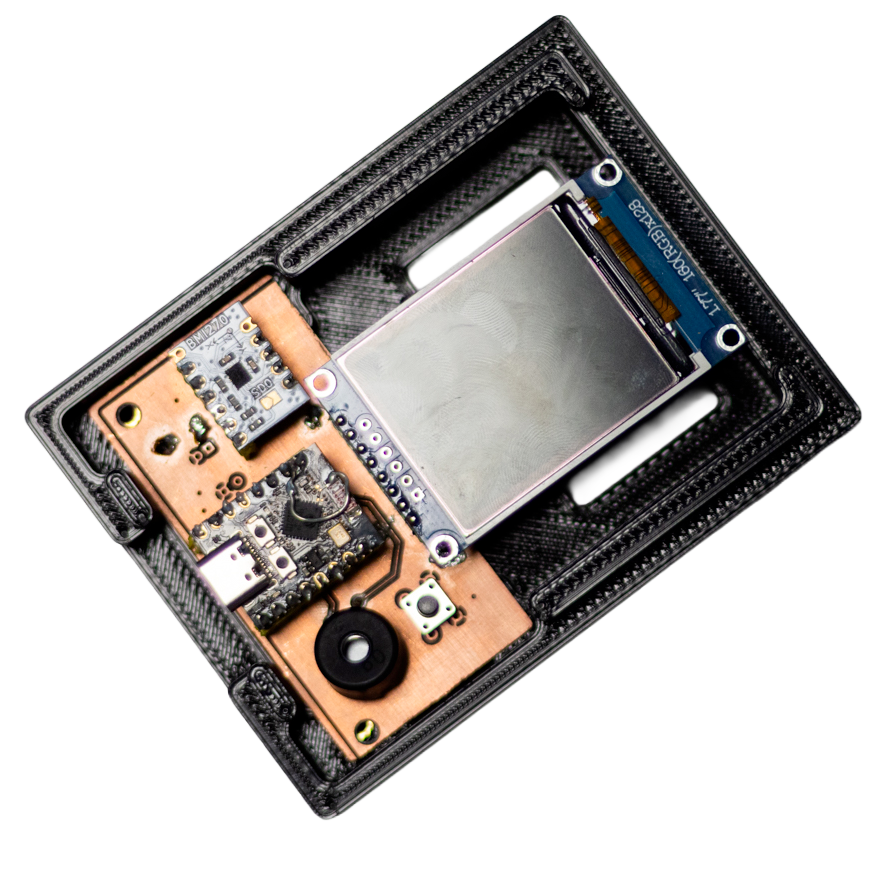
\includegraphics[width=0.49\linewidth]{pcb_box.png}
  \captionof{figure}{The enclosure: exploded render of the three printed parts from their STL files (left) and the assembled PCB inside the printed box (right).}
  \label{fig:boxmain}
\end{colfig}

\paragraph{Start sequence.}
A press starts a 3~s countdown, then ``on your marks''; ``set'' follows 20--25~s later. The unit then waits until the sprinter is measured still (horizontal acceleration under 15~mg for 200~ms) and fires ``go'' a random 0.7--1.5~s later, which makes ``go'' hard to anticipate. Each beep is a 4~kHz, 100~ms tone and introduces no software latency into the reaction time.

\paragraph{Onset detection.}
The BMI270 runs at 800~Hz nominal (803.6~Hz measured), $\pm$16~g. Gravity is estimated at rest as a vector, so every sample splits into vertical and horizontal parts whatever the mounting angle. An STA/LTA trigger \cite{allen} (15/800~ms windows, ratio 6, 20~mg floor) decides that the athlete moved; Maeda's AIC picker \cite{maeda} then finds, from 150~ms before to 50~ms after the trigger, the sample that best splits a quiet segment from an active one, and reports it as the onset. Because this second step has no threshold, the onset does not move with the trigger level: across 79 starts and thresholds of 10--50~mg it stayed on the same sample in 70 starts and within one in 74, while a threshold-only detector drifted by a median 9.3~ms (Appendix~\ref{app:sweep}). After the result, the unit sends the run to the app over BLE, which saves it as CSV; the board keeps it in RAM until the app confirms.

\paragraph{App and clock synchronization.}
The Flutter app (iOS) connects to the unit's GATT service. In \emph{Reaction} mode it mirrors the unit's phases and shows the reaction time. In \emph{Photofinish} mode it also times the finish and reports total, reaction and run time (Figure~\ref{fig:app}); for this, the board's ``go'' instant must be converted to the phone's clock, so the app estimates the offset $\theta$ (phone time minus board time). Between ``on your marks'' and ``set'' the phone pings the board for 10~s. Each ping has four timestamps: the phone sends at $t_1$, the board receives at $t_2$ and replies at $t_3$, and the phone receives at $t_4$. Each one-way difference equals $\pm\theta$ plus a transmission delay that varies but is never negative, so the smallest value in each direction is the least noisy:
\[
a=\min(t_2-t_1),\quad b=\min(t_4-t_3),\quad \theta=\tfrac{b-a}{2}.
\]
The two directions are minimized separately because BLE delays are asymmetric: a reply waits for the next connection event, which can skew a single round trip by up to one interval (15--30~ms on iOS) \cite{cristian}. The offset error is bounded by half the minimum round trip, $(a+b)/2$, which the app computes on every sync. On an iPhone~13 this bound was 19~ms, set by the $\sim$30~ms iOS connection interval (forcing 15~ms had no effect). The bound is conservative, as it assumes the entire minimum delay falls in one direction; the end-to-end photofinish comparison (Sec.~\ref{sec:eval}) suggests the actual error is considerably smaller. Clock drift (20--50~ppm) adds under 0.5~ms between sync and start.

\begin{colfig}
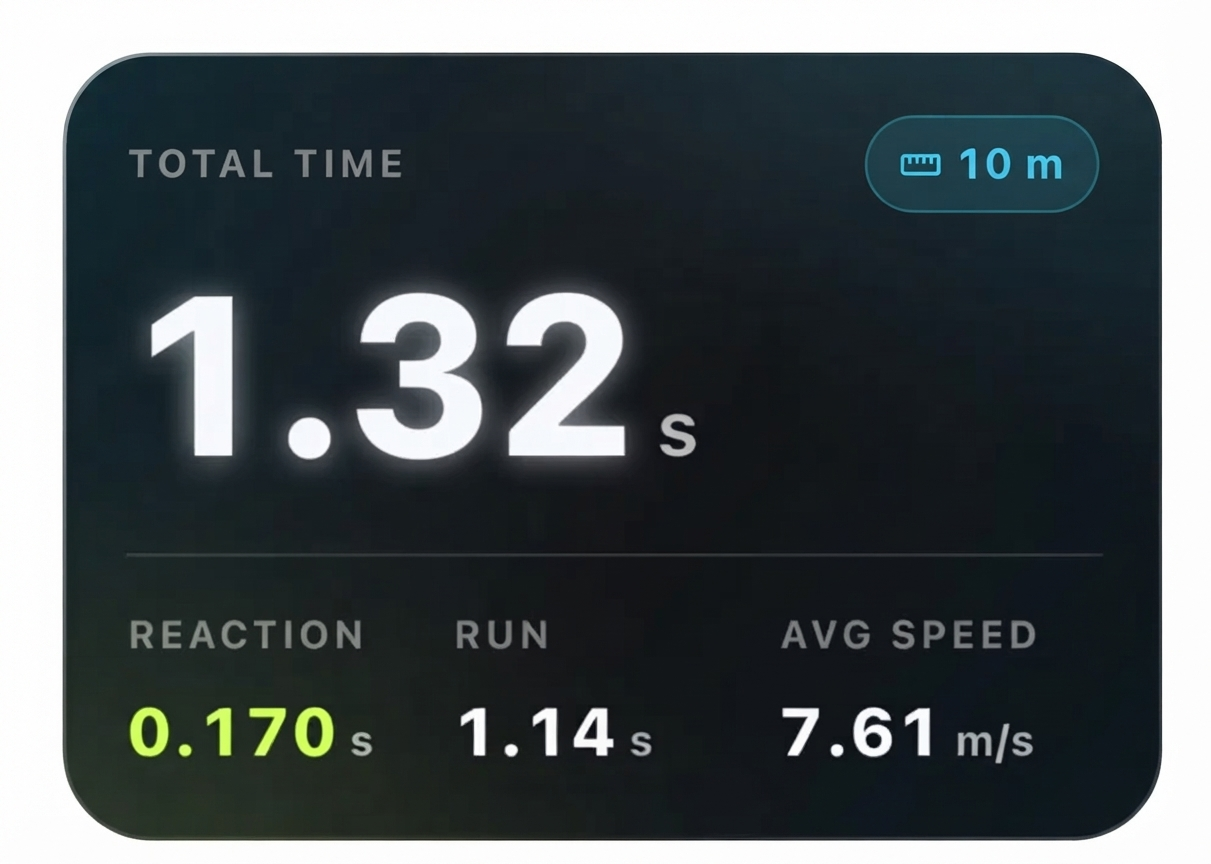
\includegraphics[width=\linewidth,height=3.8cm,keepaspectratio]{appscreen.jpg}
\captionof{figure}{The app's result screen after a 10~m run on an iPhone~13.}
\label{fig:app}
\end{colfig}

\paragraph{Camera-based photo finish.}
The phone stands in line with the finish, and the user drags a line onto the real one. The camera runs at its highest frame rate (240~fps on an iPhone~13), with no stabilization and a short exposure (1/1000~s) against motion blur; every frame keeps the time it was captured, on the same clock the synchronization uses. From ``go'' the frames are kept in memory, and when a body enters a narrow band around the line, MediaPipe Pose \cite{blazepose} analyzes the pass. The rules time the torso \cite{watr}, but the pose landmarks are joints inside the body, so the center of the torso crosses about 20~ms after the chest. We therefore take the chest front from the body silhouette: between shoulders and hips, with the arm removed, the frontmost edge of each row, and the 80th percentile of these edges, so a stray forearm cannot move it. Between the last frame before the line and the first after it, interpolation gives the crossing instant, and a line fit over $\pm$160~ms smooths per-frame noise. The time is shown to the millisecond and, as the rules prescribe, rounded up to the hundredth \cite{watr}. The detector was first written in Python and then ported to the app; on the same clips the two agree within a few ms (0.864 vs.\ 0.862~s at 240~fps).


%% =====================================================================
\section{Evaluation \& Results}
\label{sec:eval}
%% =====================================================================

\paragraph{Timing path.}
On the PCB the unit samples at 803.6~Hz with no gaps and no dropped samples, a maximum interval of 1.25~ms, and 0.55~$\mu$s timestamp jitter. Re-running the detector offline on every capture gives the board's onset on the same sample (e.g.\ 163.8~ms). The unit's own resolution is therefore one sample, 1.2~ms. Figure~\ref{fig:start} shows what the detector sees in a block start.

\begin{colfig}
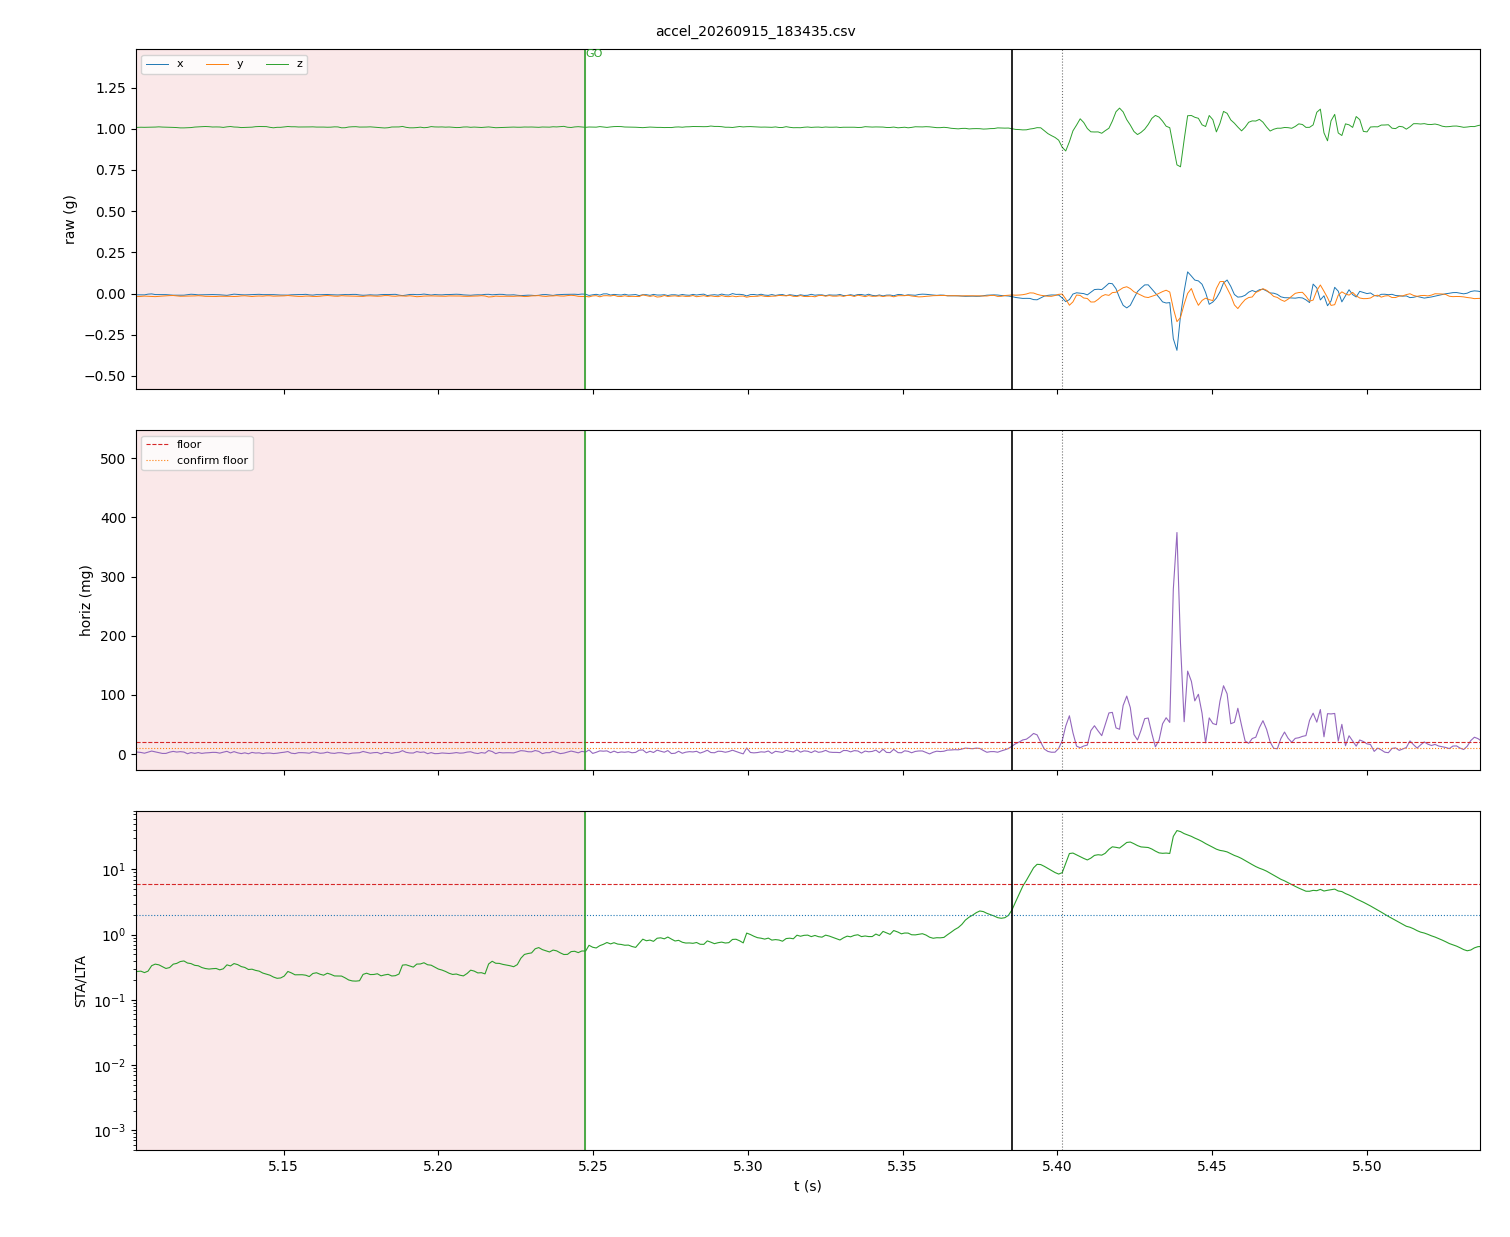
\includegraphics[width=\linewidth]{start_138ms.png}
\captionof{figure}{A block start recorded with the first prototype: raw acceleration, horizontal magnitude and STA/LTA ratio after ``go'' (green), with the AIC onset (black) at 138~ms, 16.2~ms before the threshold-only onset (dotted).}
\label{fig:start}
\end{colfig}

\paragraph{Reaction time vs.\ 240~fps video.}
As an independent reference, we filmed the block at 240~fps (4.2~ms per frame) during test starts and took the reaction time from the footage as the interval between the ``go'' signal and the push-off. The ``go'' instant is the first frame in which the green LED is lit. The push-off is harder to place: the shoe starts to compress against the block before the athlete visibly moves, so the frame was chosen by eye and may be off by a frame or two. Figure~\ref{fig:validation} shows the two video frames for an example start and the board's reading.

\begin{colfig}
\centering
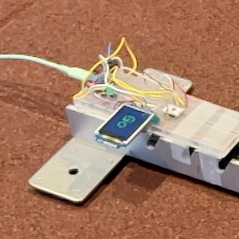
\includegraphics[width=0.32\linewidth]{1.png}\hfill
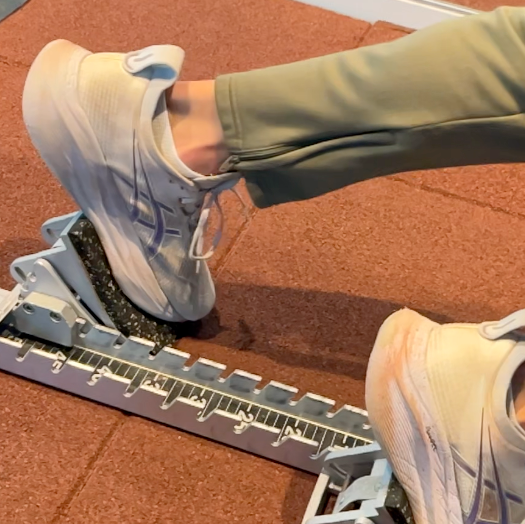
\includegraphics[width=0.32\linewidth]{2.png}\hfill
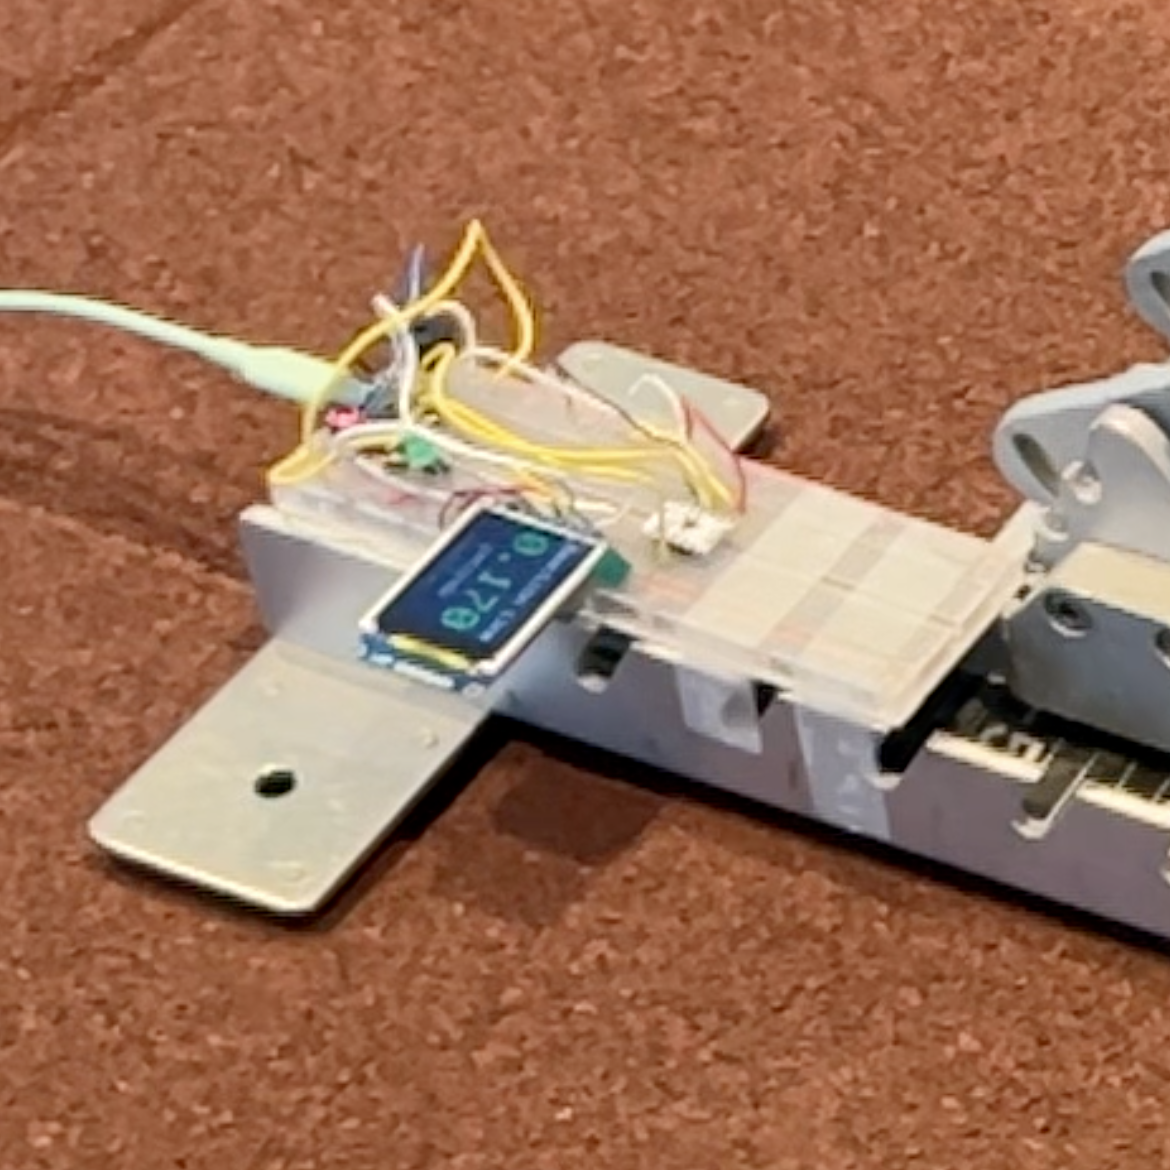
\includegraphics[width=0.32\linewidth]{3.png}
\captionof{figure}{Example start: the ``go'' frame with the green LED lit (left), the push-off frame at 240~fps (middle), and the reaction time shown by the prototype (right).}
\label{fig:validation}
\end{colfig}

Board and video agreed within about 8~ms, roughly two frames. The buzzer was about 1.5~m from the athlete, so the sound arrives about 4.4~ms after ``go'' (at 343~m/s). This is a systematic offset, and for a known distance it can be subtracted. The board's error is therefore at most about 8~ms, a bound set by the video reference itself; with a sharper reference, we expect it to approach the 1.24~ms sampling interval of the accelerometer.

\paragraph{Photo finish.}
The finish time depends on the clock synchronization between the unit and the phone, the camera frame timestamps and the crossing detector, so we validated them together, end to end. In a test run against a 60~fps reference video read frame by frame, the app's finish time differed by 10~ms. This is less than one frame of the reference video (16.7~ms) and well within the 33~ms (one frame at 30~fps) target set at the design stage. As with the reaction time, the reference cannot resolve differences much below one frame, while the app interpolates between the frames surrounding the line to obtain a sub-frame crossing time (Figure~\ref{fig:finishframe}); more runs are needed to characterize its error. We also timed the same run by hand: the stopwatch read about 0.2--0.3~s faster than the app, in line with the 0.24~s reported in the literature \cite{mann}.

\begin{colfig}
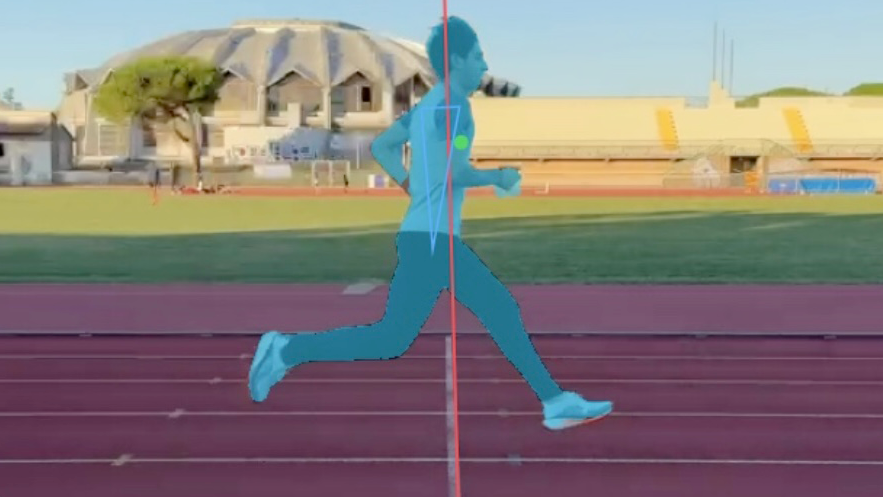
\includegraphics[width=0.8\linewidth,keepaspectratio]{figures/detection.png}
\captionof{figure}{The app's result frame at the crossing: finish line, body silhouette (cyan) and the timed chest point.}
\label{fig:finishframe}
\end{colfig}

\paragraph{Limitations.}
The validation is preliminary: the finish time rests on a single run, and both video references bound the error rather than measure it; a finer validation is planned. Besides the constant delays, the direct BLE link reaches about 30~m, so a full 100~m needs the relay planned in Section~2. In low light the exposure cannot go below about 1/250~s, increasing motion blur. An arm across the chest can hide the chest edge, and with two athletes in frame the detector times the larger torso, so the app is meant for one athlete per run.


\section{Conclusions}
%% =====================================================================

We built a start unit on one microcontroller, from PCB to printed box, and a phone app that together time a sprinter's reaction and finish, for about 300~SEK in parts (Table~\ref{tab:bom}), against about US\$1{,}600 for a single-block commercial trainer \cite{vsath}.
Against video, reaction times agreed within about 8~ms, the uncertainty of the reference itself, and a first finish time within 10~ms, whereas a stopwatch read about 0.24~s fast.
Next, a 1000~fps camera will check the unit's 1.24~ms sampling interval directly and measure the constant delays of the sensor and the sound, and the unit, now powered by a USB power bank, will move to a built-in LiPo cell.

\end{multicols}

\clearpage
{\small
\begin{thebibliography}{99}\setlength{\itemsep}{0pt}

\bibitem{vsath} VS Athletics.
\newblock ReacTime Personal Training System (SKU Z5110), Lynx.
\newblock \url{https://www.vsathletics.com/store/ReacTime-Personal-Training-System.html}, accessed 21 Sept 2026.

\bibitem{olymp} Olympics.com.
\newblock Paris 2024 athletics: Noah Lyles wins Olympic men's 100m gold in a photo finish, 2024.
\newblock \url{https://www.olympics.com/en/news/noah-lyles-wins-paris-2024-athletics-olympic-mens-100m-gold}, accessed 19 Sept 2026.

\bibitem{lipps} D.~B. Lipps, A.~T. Galecki, and J.~A. Ashton-Miller.
\newblock On the implications of a sex difference in the reaction times of sprinters at the Beijing Olympics.
\newblock \emph{PLoS ONE}, 6(10):e26141, 2011.
\newblock doi:10.1371/journal.pone.0026141.

\bibitem{pain} M.~T.~G. Pain and A.~Hibbs.
\newblock Sprint starts and the minimum auditory reaction time.
\newblock \emph{Journal of Sports Sciences}, 25(1):79--86, 2007.
\newblock doi:10.1080/02640410600718004.

\bibitem{brosnan} K.~C. Brosnan, K.~Hayes, and A.~J. Harrison.
\newblock Effects of false-start disqualification rules on response-times of elite-standard sprinters.
\newblock \emph{Journal of Sports Sciences}, 35(10):929--935, 2017.
\newblock doi:10.1080/02640414.2016.1201213.

\bibitem{lynx} FinishLynx.
\newblock ReacTime false start detection system.
\newblock \url{https://www.finishlynx.com/product/reactime-false-start-detection/}, accessed 21 Sept 2026.

\bibitem{mann} J.~B. Mann, P.~J. Ivey, W.~F. Brechue, and J.~L. Mayhew.
\newblock Validity and reliability of hand and electronic timing for 40-yd sprint in college football players.
\newblock \emph{Journal of Strength and Conditioning Research}, 29(6):1509--1514, 2015.
\newblock doi:10.1519/JSC.0000000000000941.

\bibitem{haugen} T.~A. Haugen, E.~T{\o}nnessen, and S.~K. Seiler.
\newblock The difference is in the start: impact of timing and start procedure on sprint running performance.
\newblock \emph{Journal of Strength and Conditioning Research}, 26(2):473--479, 2012.
\newblock doi:10.1519/JSC.0b013e318226030b.

\bibitem{lynxpatent} E.~Widding, D.~DeAngelis, and A.~Barton (Lynx System Developers, Inc.).
\newblock Reaction time measurement system.
\newblock US Patent 6,002,336, 1999. PCT publication WO~1999/032889~A2.

\bibitem{omega} OMEGA.
\newblock Official Timekeeper: a legacy of Olympic precision since 1932.
\newblock \url{https://www.omegawatches.com/en-us/world-of-omega/olympic-and-paralympic-games/official-timekeeper}, accessed 21 Sept 2026.

\bibitem{heim} F.~Heim, I.~R. Kristinsson, A.~Rosato, and M.~Zimmermann.
\newblock Design of a sprint block for force and reaction time measurement.
\newblock Course paper, November 2020.

\bibitem{allen} R.~V. Allen.
\newblock Automatic earthquake recognition and timing from single traces.
\newblock \emph{Bulletin of the Seismological Society of America}, 68(5):1521--1532, 1978.

\bibitem{maeda} N.~Maeda.
\newblock A method for reading and checking phase times in auto-processing system of seismic wave data.
\newblock \emph{Zisin (Journal of the Seismological Society of Japan)}, 38(3):365--379, 1985.

\bibitem{cristian} F.~Cristian.
\newblock Probabilistic clock synchronization.
\newblock \emph{Distributed Computing}, 3(3):146--158, 1989.
\newblock doi:10.1007/BF01784024.

\bibitem{blazepose} V.~Bazarevsky, I.~Grishchenko, K.~Raveendran, T.~Zhu, F.~Zhang, and M.~Grundmann.
\newblock BlazePose: on-device real-time body pose tracking.
\newblock \emph{CVPR Workshop on Computer Vision for Augmented and Virtual Reality}, 2020. arXiv:2006.10204.

\bibitem{watr} World Athletics.
\newblock Competition Rules, Book C2.1: Technical Rules, Rule 19 (Timing and Photo Finish).
\newblock \url{https://worldathletics.org/about-iaaf/documents/book-of-rules}, accessed 18 Oct 2026.

\bibitem{bmi} Bosch Sensortec.
\newblock BMI270: 6-axis smart, low-power inertial measurement unit, datasheet.
\newblock \url{https://www.bosch-sensortec.com/products/motion-sensors/imus/bmi270/}, accessed 18 Oct 2026.

\end{thebibliography}
}

\clearpage
\appendix
\section{Source code}
\label{app:code}

Everything needed to rebuild the system is in one repository, \url{https://github.com/lorenzogalli-dev/Prostart}:

\begin{table}[H]
\centering\small
\begin{tabularx}{\linewidth}{lL}
\toprule
Folder & Content \\
\midrule
\texttt{Arduino/AlgorithmRealTimeESP32/} & start-unit firmware (ESP32-C3 + BMI270, BLE); wiring, build and test notes \\
\texttt{Arduino/AlgorithmRealTime/} & first prototype (XIAO nRF52840 Sense), same detector \\
\texttt{Arduino/EspNowLrTest/} & long-range ESP-NOW field test for the finish relay, with its measurements \\
\texttt{prostart/} & Flutter app and its native camera plugin (photo finish) \\
\texttt{AI\_Torso\_Detector/} & Python reference of the photo-finish detector (MediaPipe) \\
\texttt{Hardware/} & KiCad project, Gerbers and BOM (\texttt{PCB\_ProStart\_POC/}); enclosure STL files (\texttt{Enclosure/}) \\
\texttt{Data/}, \texttt{Arduino/*/Data/} & recorded block starts (CSV), used for the threshold sweep (Appendix~\ref{app:sweep}) \\
\bottomrule
\end{tabularx}
\caption{Repository layout.}
\label{tab:repo}
\end{table}

\section{Hardware}
\label{app:hw}

The first prototype (Figure~\ref{fig:prototype}) was a Seeed XIAO nRF52840 Sense, whose on-board LSM6DS3 accelerometer sampled at about 865~Hz, with a button and the buzzer on a breadboard; it recorded the 79 block starts of Appendix~\ref{app:sweep} and validated the detector. The final unit moves to an ESP32-C3 with an external BMI270, whose FIFO decouples sampling from the radio, on a custom two-layer PCB (Figures~\ref{fig:schematic} and~\ref{fig:pcb}). Table~\ref{tab:bom} lists the parts, the pin map and their cost.

\begin{figure}[H]
\centering
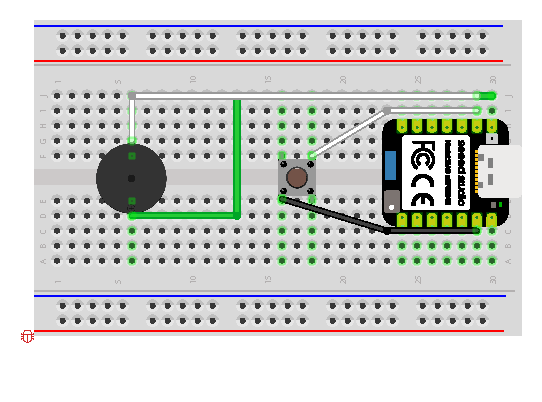
\includegraphics[width=0.48\linewidth,height=4.6cm,keepaspectratio]{prototype.pdf}\hfill
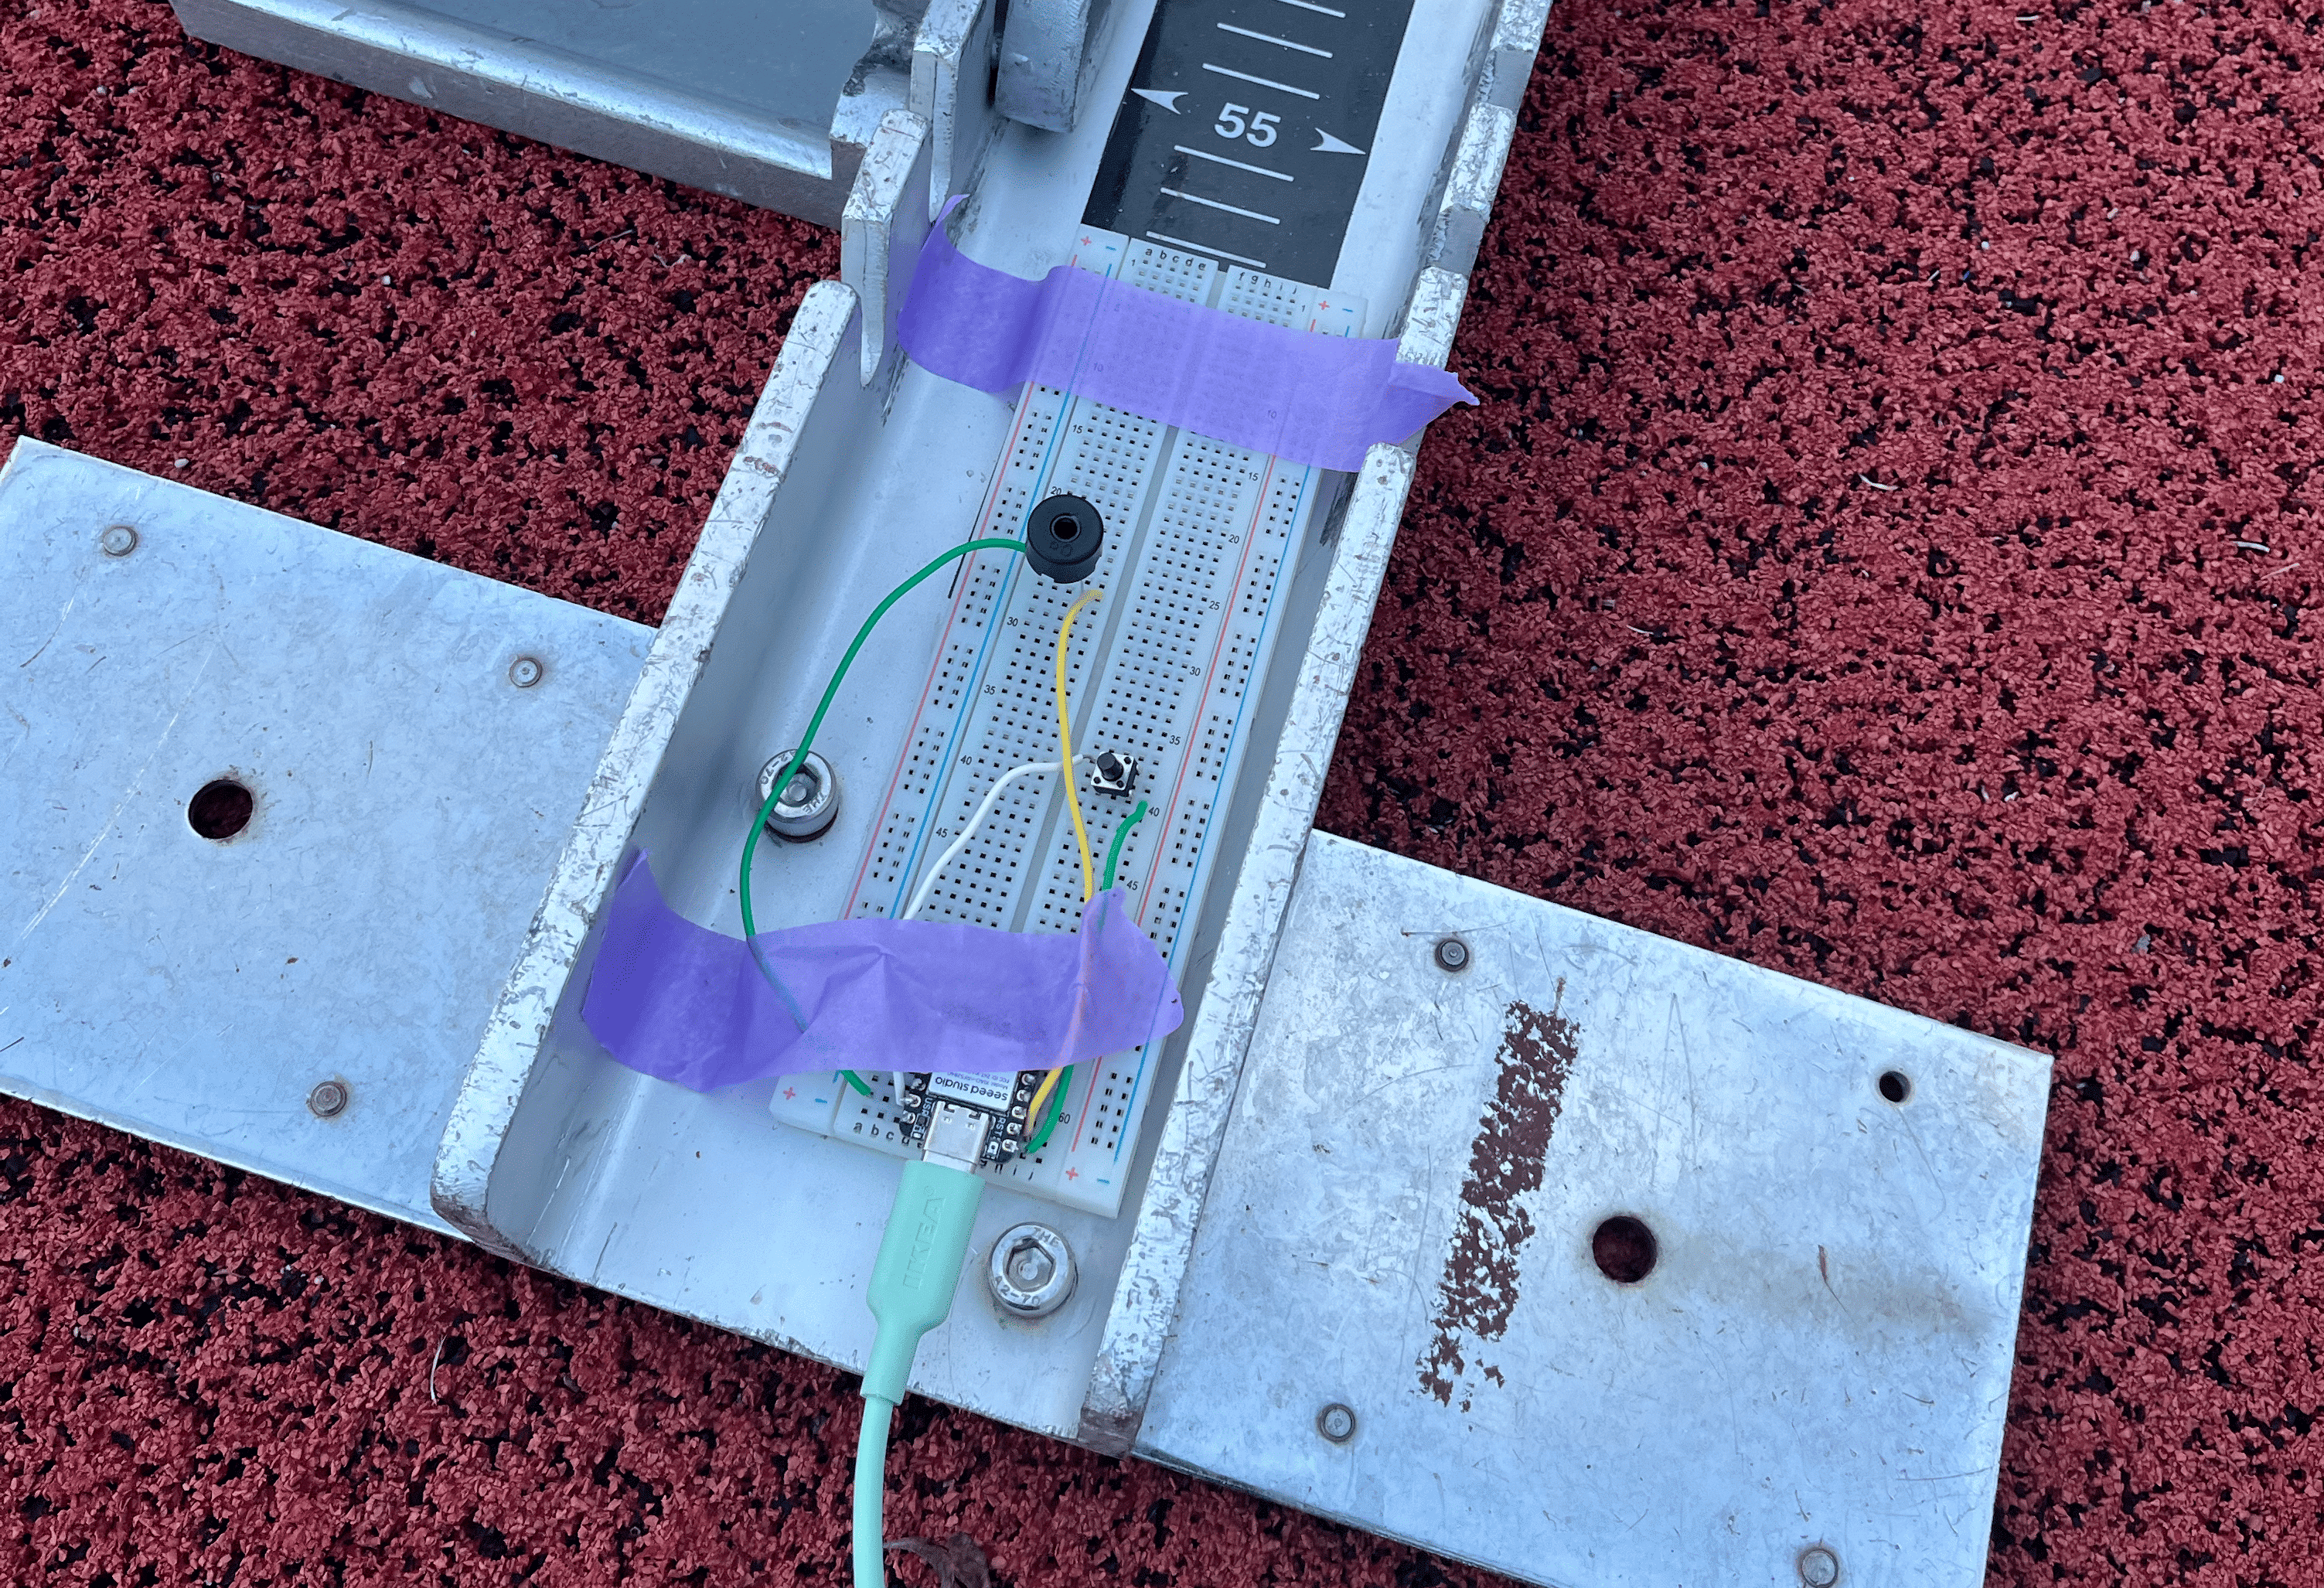
\includegraphics[width=0.48\linewidth,height=4.6cm,keepaspectratio]{prototype.png}
\caption{The first prototype: breadboard wiring diagram (left) and the real breadboard with the XIAO nRF52840 Sense, button and buzzer (right).}
\label{fig:prototype}
\end{figure}

\begin{figure}[H]
\centering
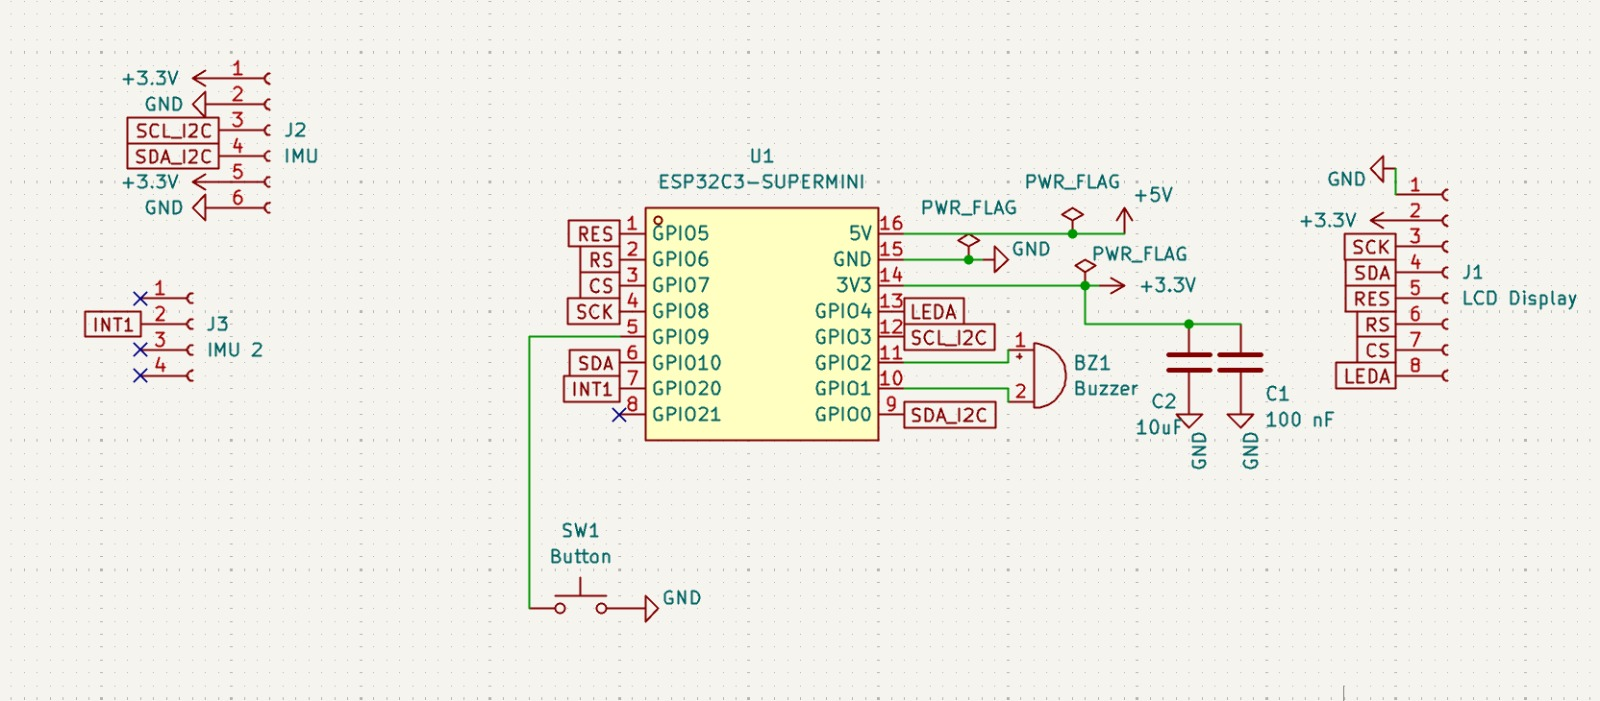
\includegraphics[width=0.48\linewidth,height=4.6cm,keepaspectratio]{pcb_schematic.jpeg}\hfill
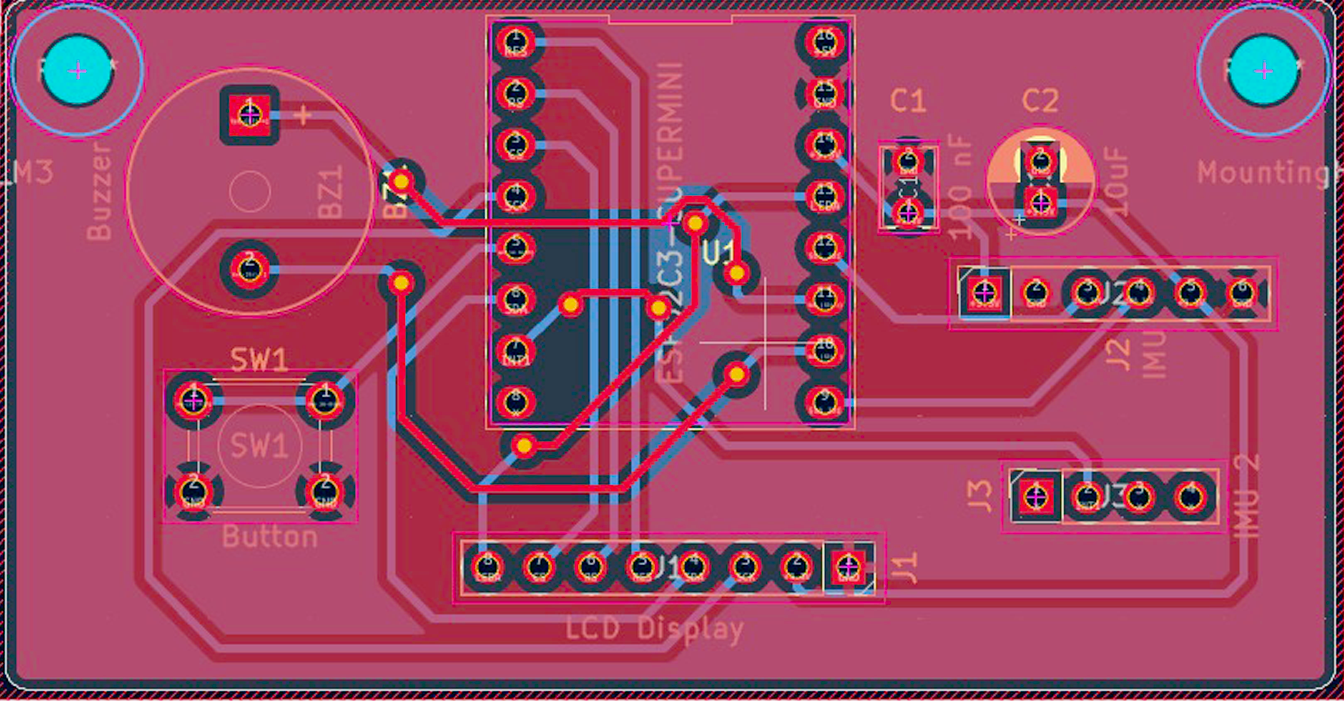
\includegraphics[width=0.48\linewidth,height=4.6cm,keepaspectratio]{pcb_layout.png}
\caption{Schematic of the start unit (left) and routed layout of the 65.5$\times$34~mm PCB (right). J2/J3: BMI270 breakout (I$^2$C, INT1); J1: TFT display; BZ1: piezo between GPIO1 and GPIO2.}
\label{fig:schematic}
\end{figure}

\begin{figure}[H]
\centering
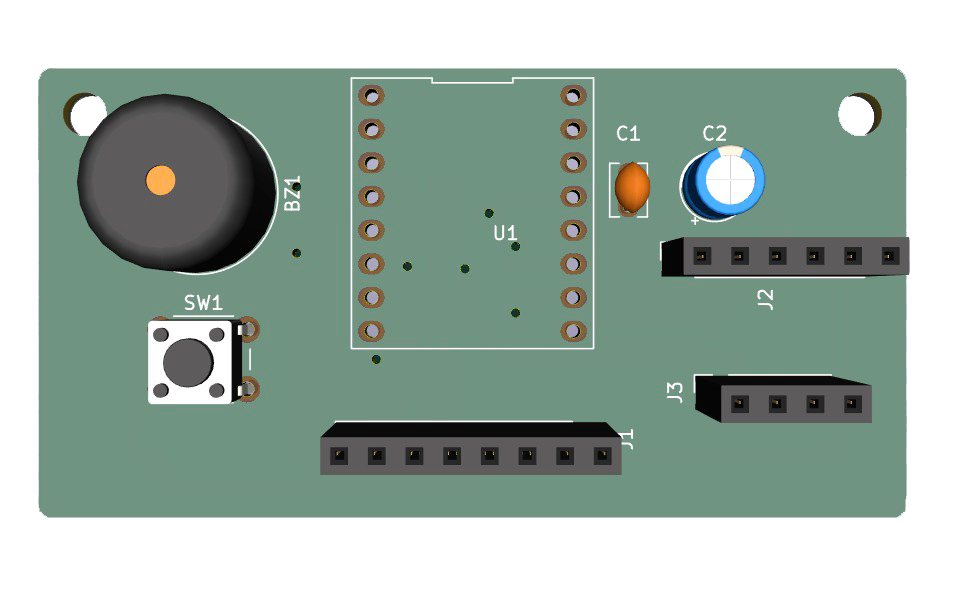
\includegraphics[width=0.48\linewidth,height=4.6cm,keepaspectratio]{pcb_3d.png}\hfill
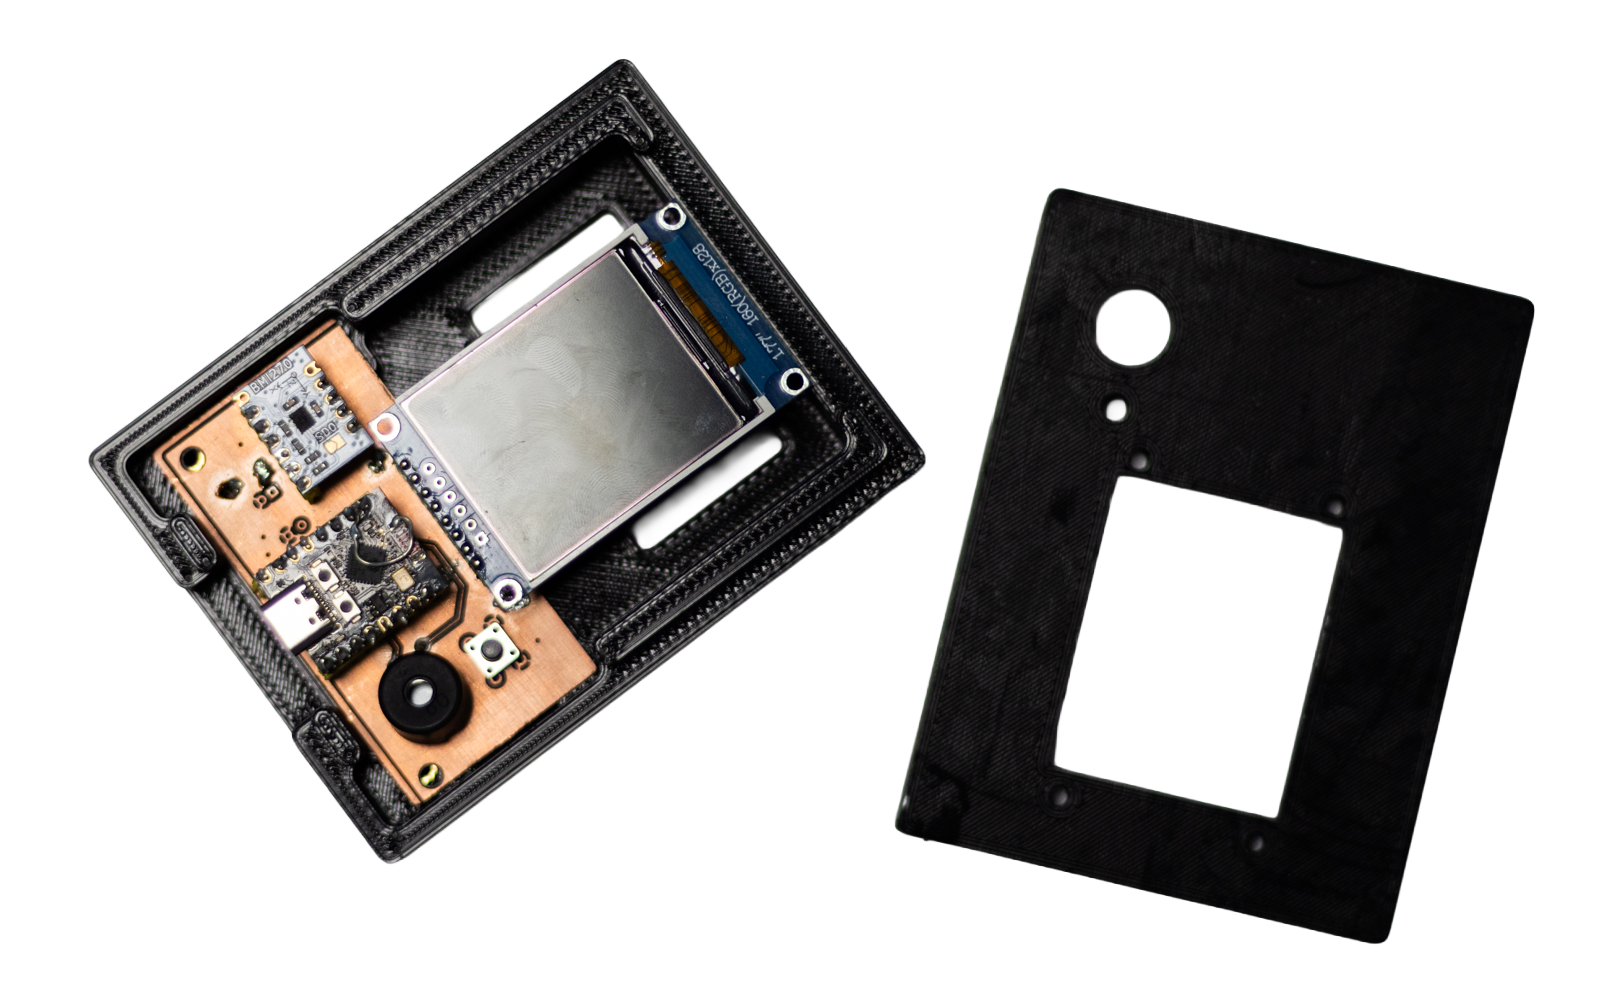
\includegraphics[width=0.48\linewidth,height=4.6cm,keepaspectratio]{pcb_open.png}
\caption{The final unit: 3D view of the PCB (left) and the assembled board with display in the printed box (right).}
\label{fig:pcb}
\end{figure}

\begin{table}[H]
\centering\small
\begin{tabular}{lllr}
\toprule
Ref. & Part & Connection & SEK\textsuperscript{*} \\
\midrule
U1 & ESP32-C3 SuperMini & -- & 40 \\
J2, J3 & BMI270 breakout \cite{bmi} & SDA GPIO0, SCL GPIO3, INT1 GPIO20 & 100 \\
J1 & 1.77'' ST7735 TFT, 128$\times$160 & SCK 8, MOSI 10, CS 7, DC 6, RES 5, BL 4 & 70 \\
SW1 & 6~mm push button & GPIO9 to GND & 5 \\
BZ1 & 12~mm piezo buzzer & GPIO1 / GPIO2, antiphase & 10 \\
C1, C2 & 100~nF, 10~$\mu$F & 3.3~V rail & 5 \\
-- & Two-layer PCB, 65.5$\times$34~mm (batch of 5) & -- & 30 \\
-- & Printed box, lid and button cap (PLA) & -- & 15 \\
-- & Strap & -- & 20 \\
\midrule
 & \textbf{Total} & & \textbf{$\approx$295} \\
\bottomrule
\end{tabular}
\caption{Bill of materials, pin map and estimated part prices. \textsuperscript{*}Estimated one-off retail prices in October 2026, excluding the phone and the USB power bank that powers the unit. The green validation LED (GPIO21, Section~\ref{sec:eval}) is not part of the product.}
\label{tab:bom}
\end{table}

\section{Firmware parameters and BLE protocol}
\label{app:params}

Table~\ref{tab:params} collects the constants of Section~2 in one place, while Table~\ref{tab:ble} is the GATT service the app talks to.

\begin{table}[H]
\centering\small
\begin{tabularx}{\linewidth}{lL}
\toprule
Parameter & Value \\
\midrule
Sampling & BMI270, 800~Hz nominal (803.6~Hz measured), $\pm$16~g, 0.488~mg/LSB; FIFO of 337 frames (0.42~s); data-ready stamped in the ISR (1~$\mu$s clock) \\
Sequence & countdown 3~s; marks $\rightarrow$ set 20--25~s; arm when $<$15~mg for 200~ms (at least 800~ms after set, at most 4~s); go 0.7--1.5~s after arming \\
Beep & 4~kHz, 100~ms, two register writes, stamped at the write \\
STA/LTA & 15~ms / 800~ms, on at ratio 6, off at 2, 20~mg floor, 15~ms confirmation \\
AIC window & 150~ms before, 50~ms after the trigger \\
False start & onset $<$ 100~ms after go \\
Timing check & before every verdict: no gap longer than 3 sample periods and no FIFO resynchronization since ``set'', otherwise the start is reported as unusable \\
Storage & none on the board: the run waits in RAM until the app confirms it has saved it \\
\bottomrule
\end{tabularx}
\caption{Start-unit parameters.}
\label{tab:params}
\end{table}

\begin{table}[H]
\centering\small
\begin{tabularx}{\linewidth}{lL}
\toprule
Characteristic & Content \\
\midrule
\texttt{event} (notify) & type, counter (a gap reveals a lost event); countdown digit; marks/set/go board time ($\mu$s); result: verdict, reaction time, onset and go times \\
\texttt{ping} (write) & 16-bit sequence number from the phone \\
\texttt{pong} (notify) & sequence, board receive time, board send time; answered only before ``set'' \\
\texttt{data} (notify) & the last start's recording: run info, samples (10~bytes each, up to 24 per packet on iOS), end of run \\
\texttt{ctrl} (write) & from the app: get a run or a range of samples; acknowledge a run once saved \\
\bottomrule
\end{tabularx}
\caption{BLE GATT service of the start unit (UUIDs \texttt{F7280000-\ldots} to \texttt{F7280005-\ldots}). Board times are 32-bit microseconds, unwrapped by the app.}
\label{tab:ble}
\end{table}

\section{Threshold independence of the onset}
\label{app:sweep}

A detector that reports the instant its signal crosses a threshold reports a later onset the higher the threshold, and on a slow push-off by several milliseconds. To check that the AIC picker does not, we re-ran the offline detector on all 79 block starts recorded with the first prototype, sweeping the detection threshold from 10 to 50~mg, once with the AIC picker and once without, and measured how far the reported onset moved from its value at the lowest threshold (Figure~\ref{fig:sweep}). The AIC onset stayed on the same sample in 70 starts and within one sample in 74, while the threshold-only onset drifted by a median 9.3~ms over the sweep. The detector's threshold therefore decides only \emph{whether} the athlete moved, not \emph{when}.

\begin{figure}[H]
\centering
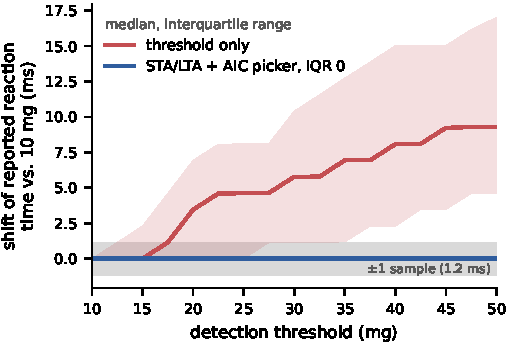
\includegraphics[width=\linewidth]{threshold_sweep.pdf}
\caption{Threshold sweep over 79 block starts recorded with the first prototype (10--50~mg): the AIC onset stays fixed while threshold-only detection drifts (median 9.3~ms).}
\label{fig:sweep}
\end{figure}

\end{document}
